\documentclass[11pt]{article}
\usepackage[utf8]{inputenc}
\usepackage[T1]{fontenc}
\usepackage{graphicx}
\usepackage[portuguese]{babel}
\usepackage{geometry}
\usepackage{listings}
\usepackage{hyperref}
\usepackage{bookmark}
\usepackage{float}
\graphicspath{ {./img/} }
\begin{document}

\title{Malha aberta}
\maketitle

\section{Modelo de simulação}
\begin{figure}[!h]
\begin{center}
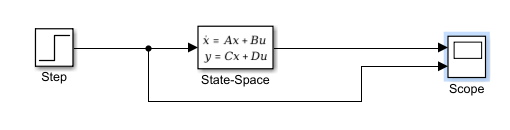
\includegraphics[width=12cm]{modelo.PNG}
\caption{Diagrama de blocos}
\label{fig1.1}
\end{center}
\end{figure}
\begin{figure}[!h]
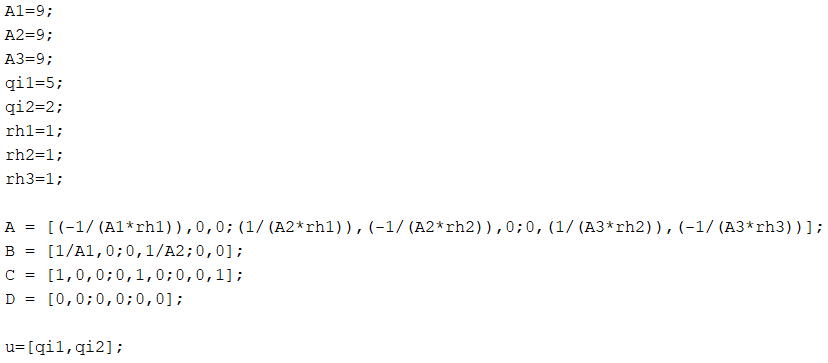
\includegraphics[width=15cm]{params.png}
\caption{Inicialização de parâmetros e matrizes}
\label{fig1.2}
\end{figure}

\pagebreak
\section{Simulações}
\subsection{Rh1=1, Rh2=1, Rh3=1}
\begin{figure}[!h]
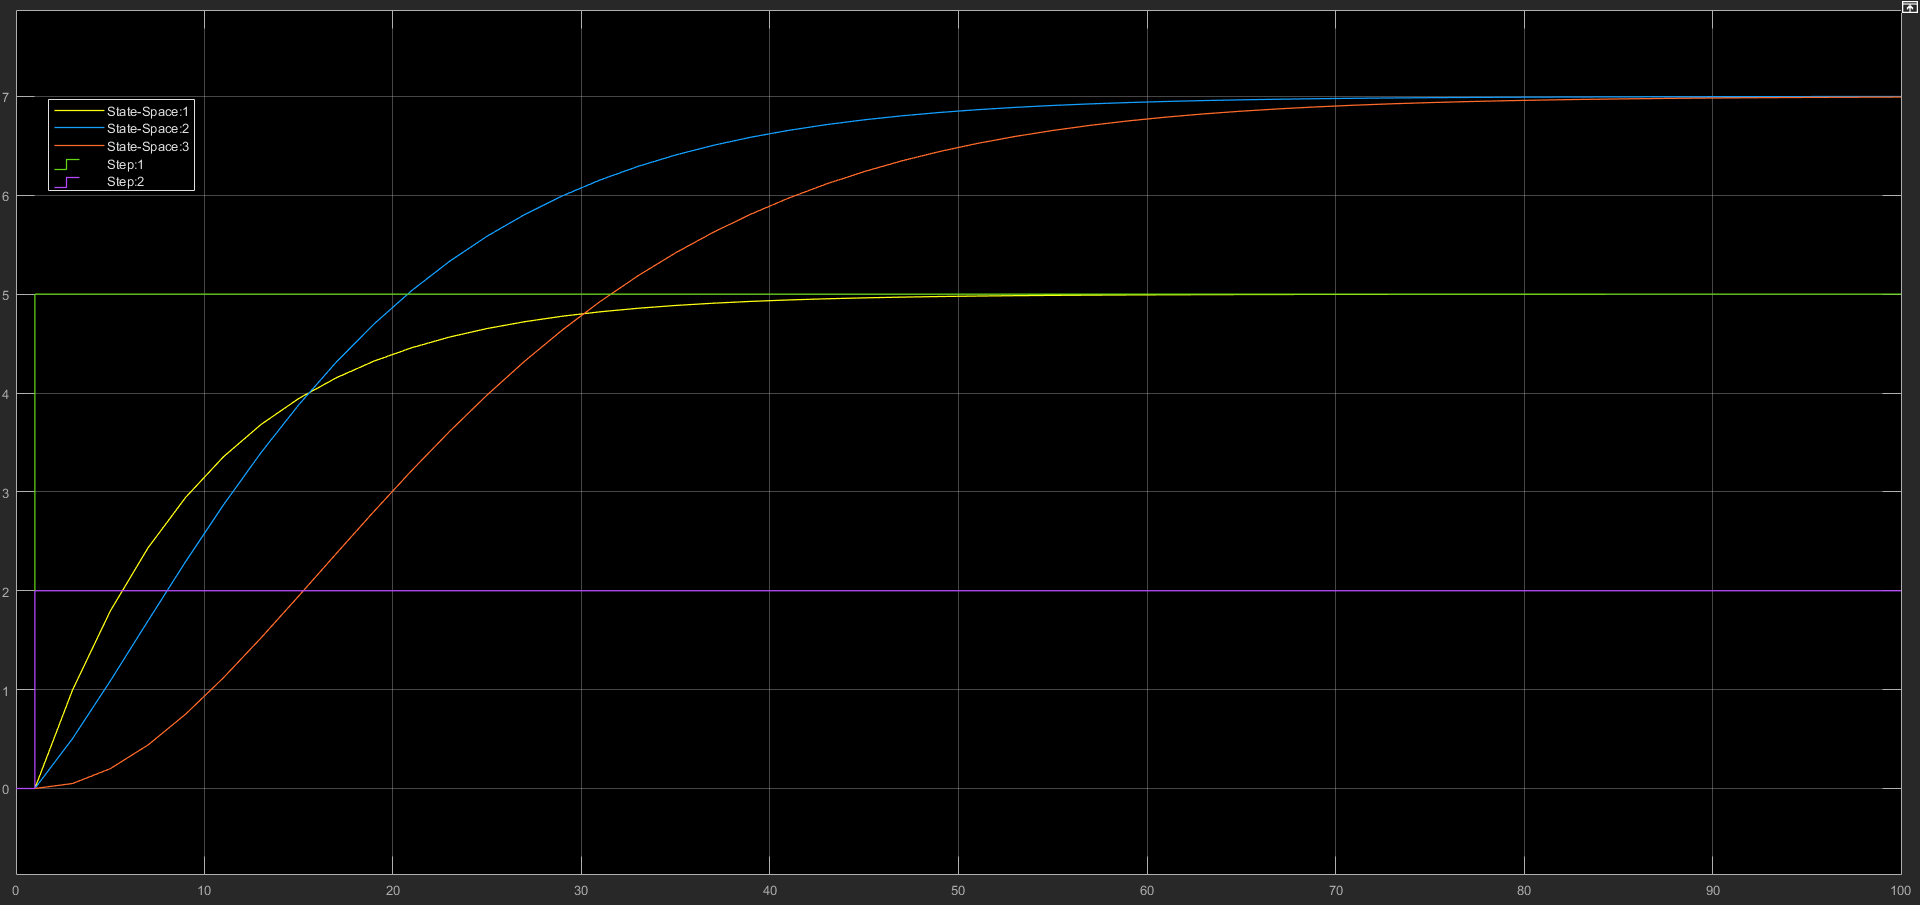
\includegraphics[width=16cm]{initial.png}
\caption{Rh1=1, Rh2=1, Rh3=1}
\label{fig2.1}
\end{figure}
Tendo todas as resistências hidráulicas como valor 1, e sabendo que qi1=5 e qi2=2, observa-se que em regime permanente h1=5, h2=7 e h3=7. h1 é o primeiro a entrar em regime permanente, seguido de h2, e  por último, h3.
\pagebreak
\subsection{Rh1=2,Rh2=1,Rh3=1}
\begin{figure}[!h]
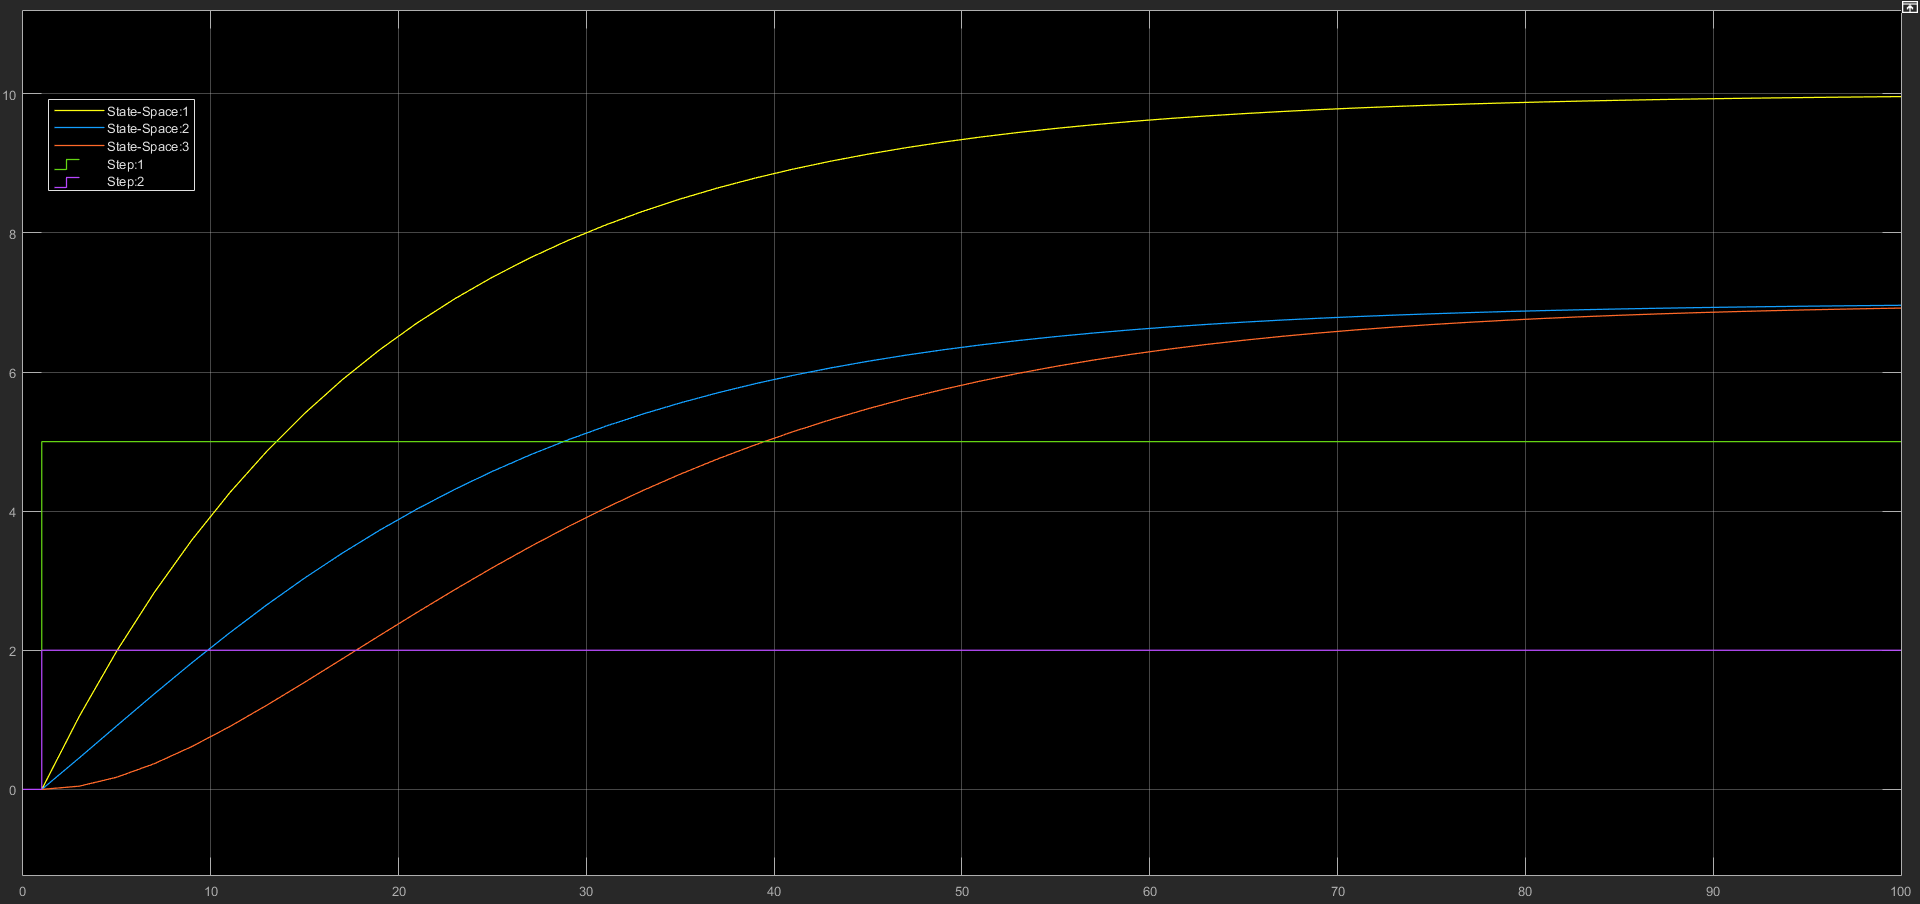
\includegraphics[width=16cm]{rh1.png}
\caption{Rh1=2, Rh2=1, Rh3=1}
\label{fig2.2}
\end{figure}
Alterando apenas o valor de Rh1 para o dobro, verifica-se uma resposta mais lenta do sistema, de forma que todas as variáveis de saída demoram mais tempo a atingir o regime permanente. Verifica-se tembém que o valor em regime permanente h2 e h3 não sofre alteração, mas o valor de h1 passa a ser o dobro, o que faz sentido uma vez que o output de água do tanque 1 passa para metade, logo acumula.
\pagebreak
\subsection{Rh1=1,Rh2=2,Rh3=1}
\begin{figure}[!h]
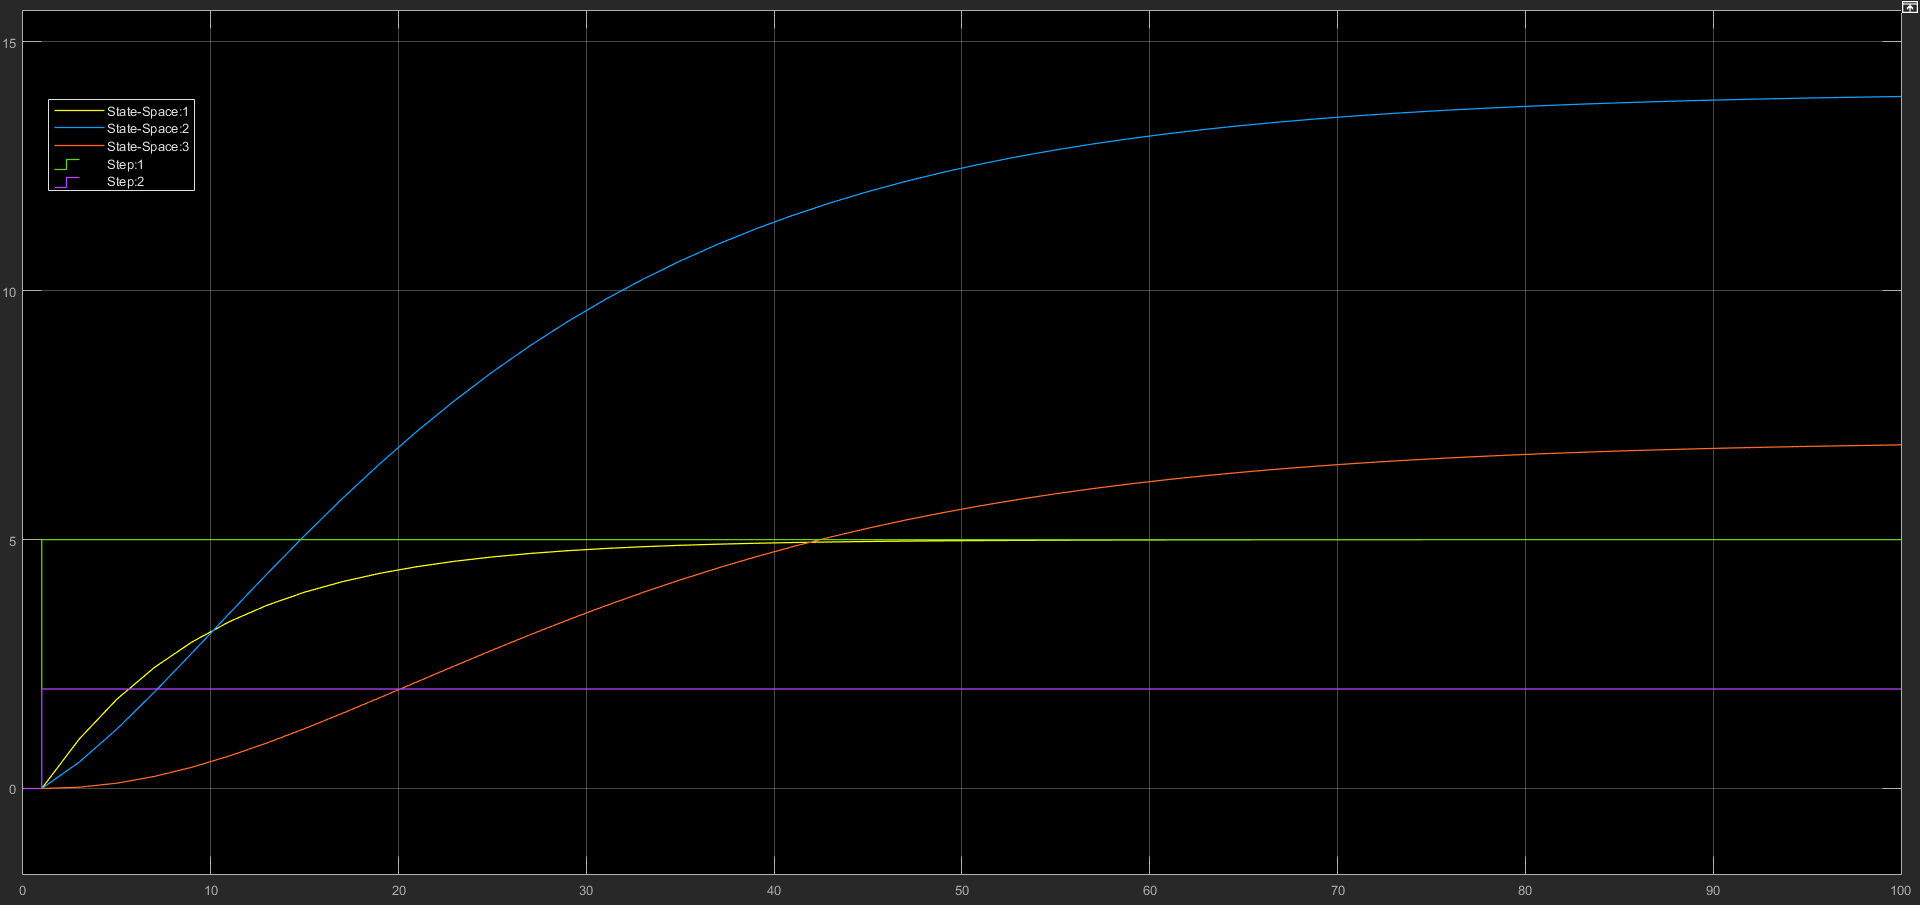
\includegraphics[width=16cm]{rh2.png}
\caption{Rh1=1, Rh2=2, Rh3=1}
\label{fig2.3}
\end{figure}
Repondo o valor de Rh1 a 1 e aumentando agr Rh2 para o dobro, verifica-se que valor de h1 não sofre qualquer alteração em nenhum estado comparativamente com a simulação inicial(\ref{fig2.1}), isto é, não altera ser valor em regime permanente, nem o tempo que demora a atingi-lo. Quanto ao valor de h2 e regime permanente, como previsto, passa para o dobro, demorando também mais tempo para o atingir. O valor em regime permanente de h3 mantém-se ainda em 7, demorando apenas mais tempo a ser atingido uma vez que o caudal de saída do tanque 2 é menor. 

\pagebreak
\subsection{Rh1=1,Rh2=1,Rh3=2}
\begin{figure}[!h]
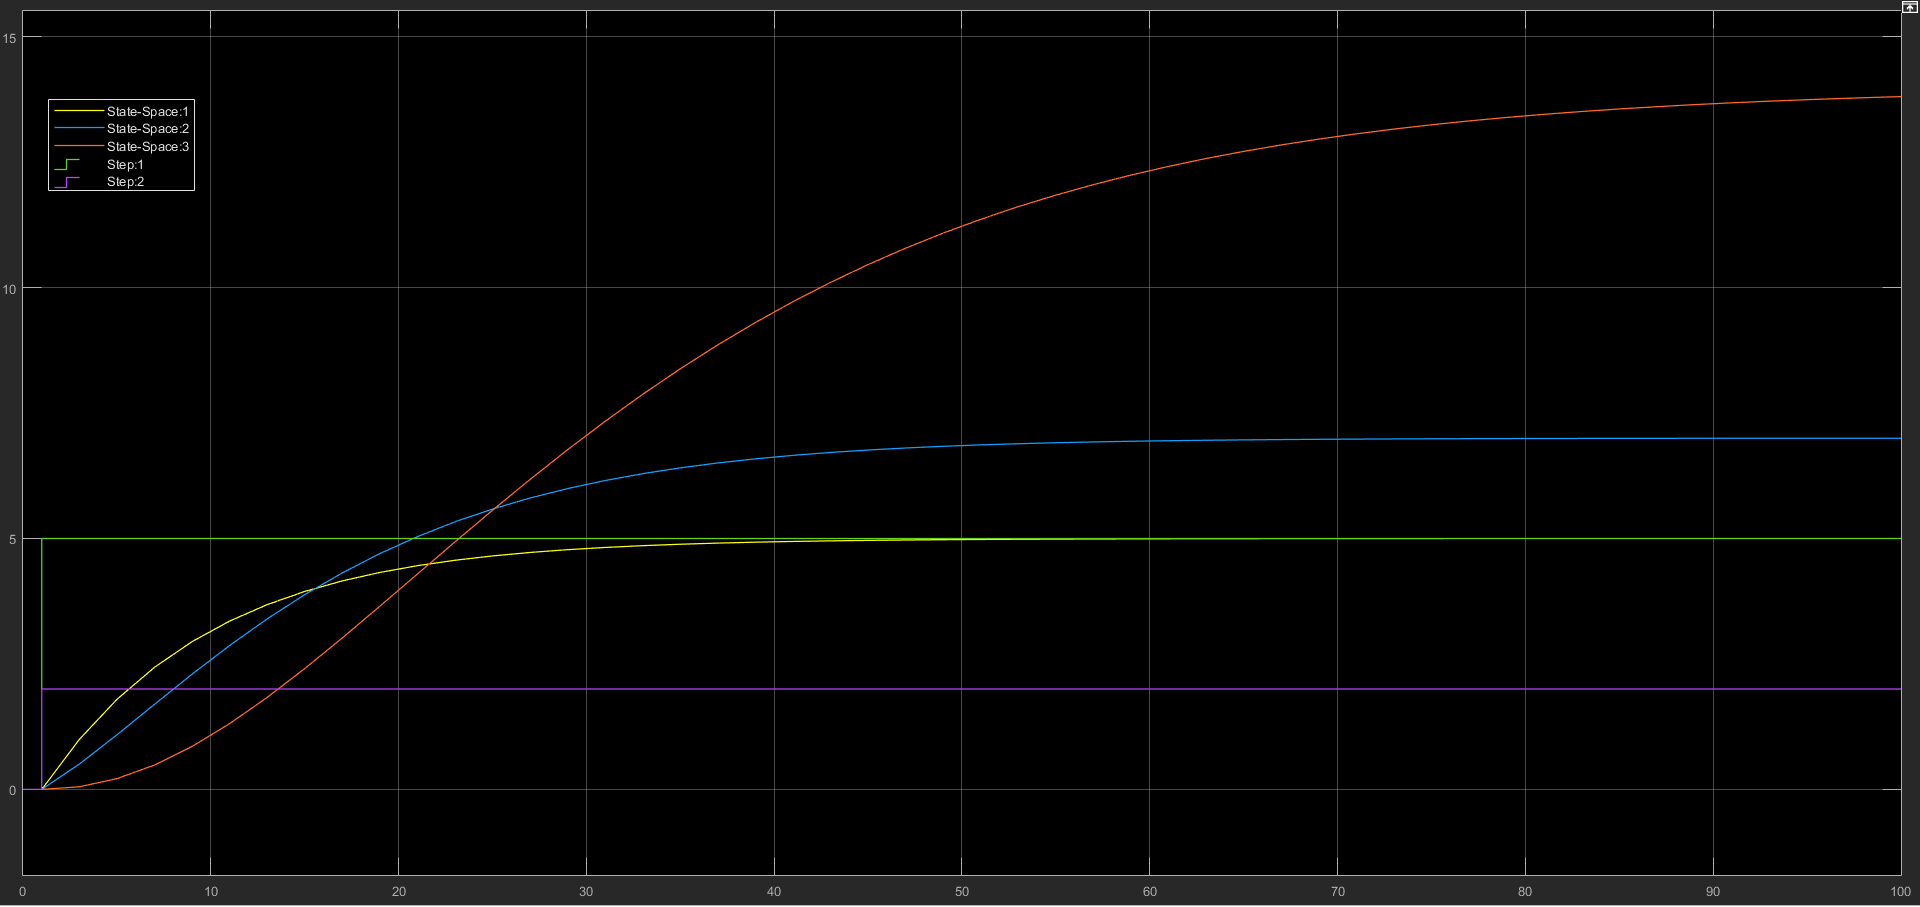
\includegraphics[width=16cm]{rh3.png}
\caption{Rh1=1, Rh2=1, Rh3=2}
\label{fig2.4}
\end{figure}
Com Rh1=1, Rh2=1 e Rh3=2 (dobro), verifica-se que h1 e h2 não sofrem quaisquer alterações em relação à simulação inicial (\ref{fig2.1}). Quanto a h3, como esperado, o seu valor em regime permanente passa para o dobro, visto que a quantidade de água que sai do tanque 3 passa para metade, e o tempo que demora atingir o regime permanente aumenta também visto que o valor que atinge é maior e tem o mesmo caudal à entrada.

\end{document}
